\documentclass[11pt,a4paper]{article}

\usepackage[margin=2.5cm]{geometry}
\usepackage{graphicx}
\usepackage{booktabs}
\usepackage{hyperref}\hypersetup{hidelinks}
\usepackage{microtype}
\usepackage{csquotes}
\usepackage[T1]{fontenc}
\usepackage{lmodern}
\usepackage[
    backend=biber,
    style=authoryear,
    maxcitenames=2
]{biblatex}

\addbibresource{references.bib}

\title{
%From citizen observations to FAIR research data:\\
%ECHOREPO and a reusable architectural pattern for soil citizen science
From citizen observations to FAIR research data:\\
ECHOREPO and a reusable architecture for soil citizen science
}

\author{Oleg Osychenko et al.\\
\small Provisional author list}

\date{Internal draft -- September 2026}

\begin{document}

\maketitle

\begin{abstract}
Citizen-science projects can generate large volumes of heterogeneous environmental data, but transforming these observations into durable research resources presents challenges that extend beyond data collection. Field observations may contain incomplete or erroneous information, geographical coordinates can raise privacy concerns, and citizen-generated records may subsequently need to be integrated with professional laboratory measurements, images, molecular biodiversity data and external research infrastructures. These requirements are often handled by project-specific pipelines that remain tightly coupled to the original data-collection application.

This paper presents ECHOREPO, an open-source and containerised research-data infrastructure developed in the context of large-scale European soil citizen science. ECHOREPO separates the acquisition layer from long-term research-data management and provides a workflow for ingestion, canonicalisation, quality assurance, provenance preservation, privacy protection, heterogeneous data enrichment and FAIR-oriented publication. The infrastructure integrates citizen observations and images with laboratory measurements and microbial biodiversity data while maintaining a common sample identity. Its production deployment currently manages around 9,000 soil samples and approximately 100 GB of data, with microbial biodiversity accounting for most of the storage and computational requirements.

Particular attention is given to problems encountered in operational citizen-science data, including erroneous or default coordinates, inconsistent observations and the need to recover rather than simply discard problematic records. ECHOREPO combines automated quality-control procedures with provenance-assisted recovery and geographical obfuscation mechanisms. Canonical research outputs are exposed through machine-readable interfaces and deposited in Zenodo with persistent identifiers and structured metadata, enabling subsequent discovery through the SoilWise infrastructure.

Rather than presenting ECHOREPO solely as a soil-specific repository, we derive a set of architectural and operational lessons relevant to other citizen-science projects seeking to transform heterogeneous participant-generated observations into FAIR, privacy-aware and reusable research data.
\end{abstract}

\vspace{0.5cm} % Adds space between abstract and keywords
\noindent \textbf{Keywords:} citizen science; FAIR data; research data infrastructure; soil monitoring; data quality; privacy; provenance; interoperability; open-source software


\section{Introduction}

% Citizen science increasingly contributes to environmental monitoring by enabling observations to be collected across geographical and temporal scales that would be difficult to achieve using professional monitoring alone. Soil monitoring is particularly well suited to participatory approaches because many relevant observations can be made in the field using relatively simple protocols, while physical samples can subsequently be subjected to professional laboratory or molecular analysis.
Citizen science has become an established approach for collecting
scientific observations across spatial and temporal scales that would
often be difficult to achieve using professional monitoring alone
\parencite{bonney2009citizenscience,bonney2014nextsteps}.

The resulting data lifecycle, however, is considerably more complex than the collection stage alone suggests. A participant may create a soil observation containing geographical coordinates, photographs and qualitative or semi-quantitative measurements. The corresponding physical sample may later undergo laboratory analysis, while a subset of samples may additionally be processed for microbial biodiversity. These data are produced at different times, by different actors and through different technical systems, yet they ultimately need to remain associated with the same research object.

Citizen-generated environmental data also introduce practical data-quality problems. Coordinates may be missing, implausible or inadvertently replaced by defaults; values may be incomplete or inconsistent; observations may be produced using different devices and languages; and the precise geographical information associated with a sample may need to be protected before public dissemination. Importantly, a quality-control system that merely removes problematic observations can result in unnecessary loss of potentially recoverable data.

These requirements suggest that a citizen-science data repository should not be treated simply as the backend database of a mobile or web application. The participant-facing acquisition system and the long-term research-data infrastructure have different requirements and lifecycles. Acquisition software may change technologies, authentication systems or interfaces during a project, whereas research data must remain identifiable, traceable, quality controlled and reusable beyond the lifetime of the collection application.

Existing citizen-science infrastructures demonstrate different approaches
to managing this data lifecycle. CitSci.org provides configurable tools
for data collection, quality assurance, metadata documentation and data
sharing, with an explicit focus on improving the discoverability and reuse
of citizen-generated datasets \parencite{wang2015citsci}. Large-scale
systems such as eBird similarly demonstrate that citizen-science
infrastructure can extend beyond data acquisition to include curation,
quality control, analysis and open data delivery
\parencite{sullivan2014ebird}. ECHOREPO addresses a related but distinct
infrastructure problem: the long-term research repository is deliberately
decoupled from the participant-facing acquisition system and must integrate
citizen observations with subsequently generated laboratory and molecular
data while supporting provenance, privacy controls and publication aligned with the FAIR principles
of findability, accessibility, interoperability and reusability
\parencite{wilkinson2016fair}.

The specific challenge addressed here is therefore not citizen-science
data collection itself, but the construction of an independent research
repository that can receive participant-generated records from an
external acquisition system and subsequently integrate them with
professional analytical data while supporting QA, privacy and persistent
publication.

We developed ECHOREPO to address these requirements in the context of European soil citizen science. ECHOREPO is an open-source, containerised platform for browsing, processing, enriching and publishing soil observations. Its current implementation provides PostgreSQL-backed canonical storage, map-oriented exploration, laboratory and biodiversity data integration, API and machine-readable exports, object storage, authentication, multilingual support and privacy and quality-control mechanisms. The software is released under the MIT License, allowing reuse and adaptation beyond the original project.

The central design principle is decoupling between acquisition and research-data management. The participant-facing mobile application uses an independent Firebase-based backend and authentication mechanism, while ECHOREPO maintains its own ingestion, canonicalisation, storage, access-control and publication infrastructure. This separation allows the acquisition system to evolve independently while maintaining a stable research-data layer.

This paper addresses four questions:

\begin{enumerate}
    \item How can a citizen-science research infrastructure remain
    decoupled from the data-acquisition application while supporting
    long-term data management?

    \item How can heterogeneous citizen observations, images, laboratory
    measurements and molecular biodiversity data be integrated while
    preserving provenance and a common sample identity?

    \item What data-quality and privacy challenges emerge in a large-scale
citizen-science deployment, and how can they be detected and mitigated,
while allowing recoverable data-quality problems to be corrected?

    \item How can the resulting research products be made persistently
    identifiable and discoverable through external FAIR data
    infrastructures?
\end{enumerate}

Using the operational ECHOREPO deployment as a case study, we describe the architecture, data lifecycle, quality-control and recovery mechanisms, privacy model and publication workflow, and derive lessons that may be applicable to other citizen-science projects.

\section{System context and design requirements}

ECHOREPO was developed within the ECHO project
(\emph{Engaging Citizens in soil science: the road to Healthier sOils}),
funded under Grant Agreement No.~101112869. The project runs from
June 2023 to May 2027 and investigates citizen participation in soil
health monitoring across Europe. ECHO combines citizen-generated field
observations with subsequent scientific analysis and research-data
management, with the aim of supporting long-term use and reuse of the
resulting soil information \parencite{echo2023project}.

Within ECHO, ECHOREPO supports a large-scale European soil
citizen-science workflow in which the data-acquisition system and the
long-term research repository are separate components. Citizen
participants collect soil observations through the EchoSoil mobile
application, which records field observations, geographical coordinates
and images and uses its own Firebase-based backend and authentication
mechanisms.

Within this workflow, the EchoSoil mobile application provides the
participant-facing data-acquisition environment, while ECHOREPO provides
the research-data management, enrichment and publication layer.

ECHOREPO is deliberately decoupled from this acquisition environment. Rather than depending on the internal database structure or identity-management system of the mobile application, it receives data through dedicated ingestion and synchronisation processes. During ingestion, participant and sample identifiers are resolved where necessary, incoming records are validated and harmonised, and the resulting information is transformed into a canonical research-data representation.

This separation establishes a clear boundary between data acquisition and research-data management. The collection application can therefore evolve independently, while ECHOREPO provides a stable layer for quality assurance, enrichment, storage, controlled access and long-term publication. The same sample can subsequently be associated with additional resources produced outside the citizen-facing application, including laboratory measurements and microbial biodiversity data.

At the time of writing, the production deployment contains around 9,000 soil samples and manages approximately 100~GB of data. Most of the storage volume and a substantial share of the computational workload are associated with microbial biodiversity data, whereas the core citizen-observation dataset and its associated images and laboratory metadata are considerably smaller.

The principal design requirements derived from this operational context were:

\begin{itemize}
    \item independence from the internal implementation of the data-acquisition application;
    \item preservation of stable sample identity across multiple stages of the data lifecycle;
    \item support for heterogeneous resources, including field observations, images, laboratory measurements and biodiversity data;
    \item preservation of traceability between source data and canonical research products;
    \item detection, classification and, where possible, recovery of citizen-generated data-quality problems;
    \item protection of sensitive geographical information prior to public dissemination;
    \item machine-readable access and support for long-term data publication; and
    \item reproducible deployment based on open-source and containerised components.
\end{itemize}
\section{Architecture}

ECHOREPO follows a layered architecture in which data acquisition, ingestion, curation, storage and publication are treated as separate concerns. This separation was a deliberate design choice. In the ECHO workflow, citizen observations are collected outside the repository itself, through a mobile application backed by Firebase services and its own authentication model. ECHOREPO therefore does not depend on the internal structure of the collection application. Instead, it acts as an independent research-data infrastructure that receives external data, harmonises them, preserves provenance and produces reusable canonical outputs.

Figure~\ref{fig:echorepo_architecture} summarises the main architectural layers and data flows.

\begin{figure}[htbp]
    \centering
    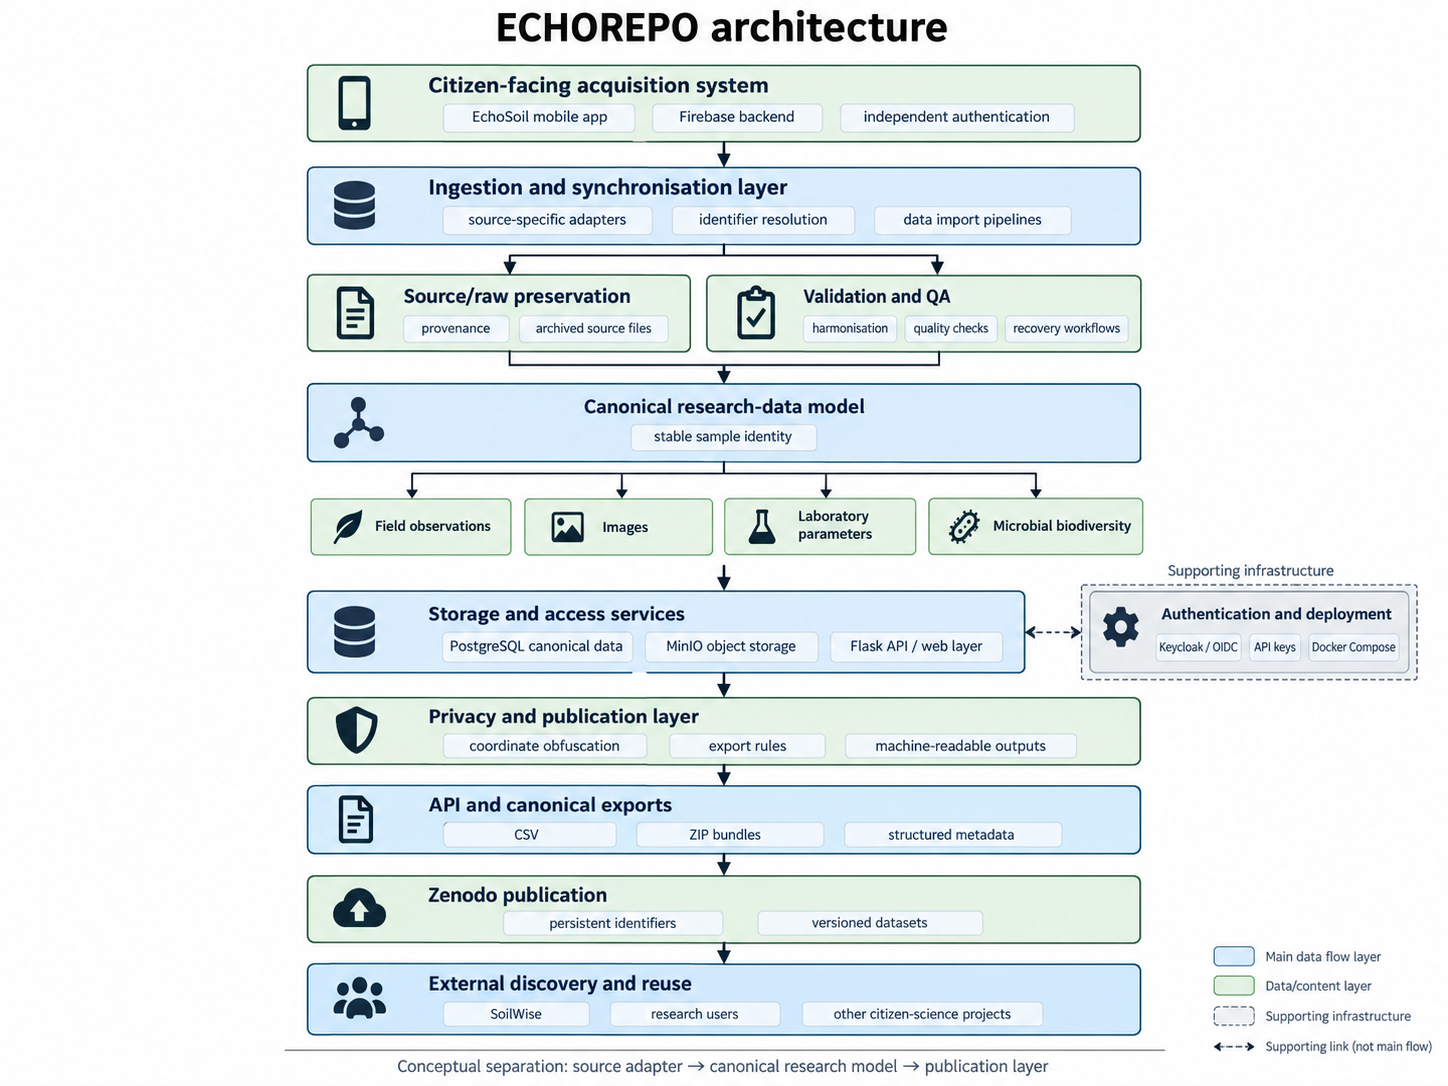
\includegraphics[width=\textwidth]{figures/echorepo_architecture_flowchart.png}
    \caption{Simplified architecture of ECHOREPO. Data are collected in an external citizen-facing system and then pass through ingestion, validation, canonicalisation, enrichment, storage and publication layers before being exposed through APIs and deposited in Zenodo for long-term FAIR dissemination.}
    \label{fig:echorepo_architecture}
\end{figure}

At the upstream end of the workflow, the citizen-facing acquisition system produces field observations, photographs and sample identifiers. These source records are imported into ECHOREPO through ingestion routines that act as adapters between the external application and the repository. A key architectural principle is that these adapters are source-specific,
while the rest of the repository is designed around a source-decoupled
canonical model. This design is intended to allow the acquisition front
end to be replaced or additional collection systems to be connected
without redesigning the downstream repository.

After ingestion, source records are preserved and subjected to validation and quality-assurance procedures. These procedures include identifier reconciliation, coordinate checking, harmonisation of heterogeneous fields, and recovery-oriented treatment of problematic citizen-generated data. Rather than simply discarding inconsistent records, ECHOREPO attempts to retain traceability and recover useful information whenever possible. This is particularly important in citizen-science settings, where data quality problems are common but often partially correctable.

The core of the system is the canonical sample model, which provides a stable representation of each sample and its associated resources. Around this core, ECHOREPO organises several linked data domains: citizen-observation attributes, sample images, laboratory parameters and microbial biodiversity data. The common sample identity maintained across these domains is essential for integrating heterogeneous evidence generated at different stages of the project.

The current implementation uses Flask for the web application and API layer, PostgreSQL for canonical structured data, and MinIO-compatible object storage for large files and immutable resources. Authentication and protected API access are handled through Keycloak/OpenID Connect together with API-key-based access mechanisms. Docker Compose is used to support reproducible deployment and operational portability. These technologies are implementation choices rather than conceptual requirements, but they demonstrate that the architecture can be realised entirely with widely available open-source components.

Before publication, canonical outputs are filtered through privacy and dissemination rules. In particular, geographical information may be obfuscated to reduce re-identification risk while retaining analytical usefulness. The resulting machine-readable resources are then exposed through the ECHOREPO API and export services, and published to Zenodo with persistent identifiers and structured metadata. This publication layer supports downstream discovery through external infrastructures such as SoilWise.

From a reuse perspective, the architecture can be understood as three main layers: a source adapter layer, a canonical research-data layer, and a publication layer. For another citizen-science project, the source adapters and parts of the canonical schema would likely need domain-specific modification, whereas much of the storage, provenance, authentication, API, publication and deployment infrastructure could be reused with comparatively limited change.
\section{Sample-centred integration of heterogeneous data}

ECHOREPO uses the soil sample as the principal entity linking heterogeneous data produced at different stages of the citizen-science workflow. Each sample is assigned a stable identifier that is retained throughout ingestion, enrichment, quality control and publication. This identifier provides the common reference needed to associate participant-generated observations with images, laboratory measurements and microbial biodiversity data.

The initial record is created during citizen participation and may contain field observations, geographical information, qualitative or semi-quantitative measurements, and photographs. Subsequent stages of the project can enrich the same sample with data generated outside the citizen-facing application. Laboratory analyses add quantitative analytical parameters, while molecular analyses introduce substantially larger biodiversity datasets, including taxonomic abundance data derived from markers such as 16S and ITS.

These data types differ considerably in structure, scale and provenance. Field observations typically consist of a relatively small number of attributes associated directly with the sample. Images are stored as separate digital objects with their own metadata. Laboratory analyses produce multiple parameter--value observations per sample, potentially using different analytical methods and units. Biodiversity analyses may generate thousands of taxonomic features and abundance measurements for a single sample. Representing all of these resources in a single flattened table would therefore introduce substantial duplication and would make provenance, schema evolution and specialist processing more difficult.

ECHOREPO instead represents the different data domains as related resources connected through the stable sample identifier. In the canonical publication model, these are exposed as separate machine-readable datasets for sample-level observations, images, laboratory parameters and biodiversity results. Supporting definition tables describe analytical parameters and methods where applicable. This relational organisation allows each data domain to evolve independently while preserving the ability to reconstruct the complete set of information associated with a sample.

The current canonical publication layer therefore follows the general structure:

\begin{itemize}
    \item \texttt{samples.csv}, containing sample-level citizen observations and geographical information;
    \item \texttt{sample\_images.csv}, describing images associated with samples;
    \item \texttt{sample\_parameters.csv}, containing laboratory and analytical measurements;
    \item \texttt{sample\_biodiversity.csv}, containing sample-associated
        microbial biodiversity results;
    \item \texttt{parameter\_definitions.csv}, describing canonical analytical
        parameters; and
    \item \texttt{analysis\_methods.csv}, describing analytical methods.
\end{itemize}

The sample-centred model is particularly important because the lifecycle of a citizen-science record does not end when the participant submits an observation. Instead, a sample may progressively acquire additional scientific information as it moves through the project:

\begin{verbatim}
citizen observation
        |
        v
field measurements + images
        |
        v
physical soil sample
        |
        v
laboratory analysis
        |
        v
microbial biodiversity analysis
        |
        v
published research resource
\end{verbatim}

These stages may occur at different times and may be performed by different organisations. Consequently, ECHOREPO must preserve not only the identity of the sample but also the provenance of the associated resources. Source files, ingestion metadata, analysis methods and timestamps are therefore retained where available, allowing published values to be traced back to the processes that produced them.

This approach also separates the logical identity of the research object from any particular acquisition or analytical system. The same sample identifier can link data originating from the citizen-facing application, laboratory workflows and biodiversity-processing pipelines, even though these systems use different data structures and operate independently. The result is a progressively enriched research object rather than a sequence of disconnected datasets.
\section{Data quality in operational citizen science}
\label{sec:data-quality}

An important lesson from operating ECHOREPO has been that citizen-generated environmental data require quality-control mechanisms that are not only automated, but also recovery-aware. In a distributed citizen-science campaign, erroneous records cannot always be prevented at the point of collection, and automatically rejecting every record that fails a validation rule may lead to unnecessary loss of otherwise valuable observations.
Data quality is consequently a recurring concern in citizen-science
projects, although appropriate validation, training and quality-assurance
procedures can produce scientifically useful datasets
\parencite{kosmala2016quality}.

In ECHOREPO, geographical information has provided a particularly useful case for developing this approach. Automated quality checks compare recorded coordinates with contextual information available for the sample, including the expected country where such information is available. They also detect coordinates corresponding to known default values and cases in which a geographical position cannot be reliably associated with a country.

A quality-assurance snapshot comprising 6,871 sample records identified 492 records (7.16\%) with coordinates classified as problematic. The detected cases consisted of 281 records for which a country could not be determined from the recorded coordinates, 123 records for which the inferred country did not match the expected country, and 88 records containing known default coordinates. Three additional records lacked planned-country information for their associated sample identifier and could therefore not undergo the same country-based validation. The distribution of QA outcomes is summarised in Table~\ref{tab:coordinate-qa}.

\begin{table}[htbp]
    \centering
    \caption{Geographical quality-control outcomes in an operational ECHOREPO data snapshot ($n=6{,}871$). Percentages are relative to the complete snapshot and are rounded to two decimal places.}
    \label{tab:coordinate-qa}
    \begin{tabular}{lrr}
        \toprule
        QA outcome & Records & Percentage \\
        \midrule
        No geographical issue detected & 6,376 & 92.79\% \\
        Country could not be determined & 281 & 4.09\% \\
        Recorded and expected country mismatch & 123 & 1.79\% \\
        Known default coordinates & 88 & 1.28\% \\
        No planned country available for validation & 3 & 0.04\% \\
        \bottomrule
    \end{tabular}
\end{table}

The first three error categories account for the 492 records marked as having problematic coordinates. The three records without planned-country information represent a different condition: the recorded coordinates were not necessarily incorrect, but one of the reference values required for the corresponding validation could not be established.

A central principle of the ECHOREPO quality-control workflow is that a failed validation check does not automatically make a sample unusable. The repository retains identifiers and provenance that can be used to investigate and, where sufficient information exists, recover problematic records. Depending on the case, this may include the sample or QR identifier, the participant associated with the sample, campaign or allocation information, expected sampling geography, and the original source record.

This is particularly relevant for coordinate errors. A sample with invalid or default coordinates may still contain valid field observations, photographs and subsequently generated laboratory data. If the sample can be reliably linked through its identifier or participant provenance to additional contextual information, its geographical information may be corrected or reconstructed without discarding the remaining scientific record.

The resulting QA process can be represented conceptually as follows:

\begin{verbatim}
incoming record
      |
      v
automated QA
      |
      +---- valid ------------------> canonical dataset
      |
      +---- flagged
              |
              v
        classify failure
              |
              v
      provenance-assisted assessment
           /       |        \
          /        |         \
     recovered   reviewed   unresolved
          |
          v
   canonical dataset
   with QA provenance
\end{verbatim}

This distinction between \emph{detection} and \emph{recovery} is important in citizen-science data management. A strict filtering strategy can improve the apparent cleanliness of a dataset, but may also discard observations whose defects affect only part of the record and can be corrected using existing provenance. ECHOREPO therefore treats quality assurance as a process of identifying, classifying and, where possible, resolving data-quality problems while preserving the relationship to the original submitted information.

The same principle extends beyond geographical information. Validation and harmonisation procedures are also required for incomplete values, inconsistent representations and heterogeneous observations produced by different participants and acquisition contexts. However, geographical QA currently provides the clearest quantitatively characterised example and is therefore used here to evaluate the operational behaviour of the recovery-aware approach.

Quantifying the effectiveness of recovery itself requires distinguishing between automatically corrected, manually reviewed and unresolved cases. These outcomes will be reported separately in the evaluation section, allowing the effectiveness of the recovery procedures to be assessed independently from the ability of the QA layer to detect problematic records.
\section{Privacy and geographical obfuscation}

Geographical information is important for environmental research because it enables observations to be associated with environmental, climatic and land-use context. In citizen science, however, precise coordinates may also disclose information about participants or sampling locations, particularly when observations are made on or near private property. ECHOREPO therefore treats geographical quality control and geographical publication as two separate stages of the data lifecycle.

Where available and operationally required, the repository first retains the best available source location in the controlled data-processing environment. Quality-assurance procedures are applied to this representation before any privacy transformation is performed. This ordering is important because an erroneous source coordinate should, where possible, be corrected before generating the public representation of the location.

For public dissemination, ECHOREPO uses spatial obfuscation rather than exposing the original sampling coordinates directly. In the current implementation, public coordinates are spatially jittered according to a configurable obfuscation radius. The production configuration uses a default radius of 1,000~m. The resulting coordinates therefore represent an approximate sampling location rather than the precise point recorded during data acquisition.

Importantly, the reduction in spatial precision is made explicit in the published data model. The canonical sample resource includes the field
\texttt{coordinate\_obfuscation\_radius\_m}, which describes the spatial obfuscation applied to the published coordinate. Downstream users can therefore distinguish an intentionally displaced public location from a measurement with metre-level positional accuracy.

Conceptually, the processing sequence is:

\begin{verbatim}
source coordinate
       |
       v
geographical validation
       |
       +---- problematic --> recovery / correction
       |                         |
       |                         v
       +----------------> best available location
                                  |
                                  v
                          privacy transformation
                                  |
                                  v
                         public coordinate
                                  +
                    obfuscation radius metadata
\end{verbatim}

This ordering separates two conceptually different operations. Quality assurance attempts to determine the most reliable geographical information available for a sample, whereas privacy protection determines how much of that information should subsequently be exposed. Consequently, correcting a coordinate does not imply that the corrected exact position must be published.

The approach aims to preserve sufficient geographical utility for regional-scale exploration and environmental analysis while reducing disclosure of exact sampling locations. It should not, however, be interpreted as a formal guarantee of anonymity. The appropriate obfuscation distance depends on the sensitivity of the data, the spatial scale of the intended analyses and the possibility of combining the published coordinates with other information.

Geographical obfuscation forms part of a broader separation between operational and public data in ECHOREPO. Personally identifying participant information is excluded from the public canonical research products, and image-processing workflows remove or suppress embedded image
metadata, such as EXIF geolocation information, that could unintentionally
disclose precise locations. Public research outputs therefore expose the scientific information required for reuse while suppressing information that is not necessary for that purpose.

Maintaining provenance internally also allows privacy protection to coexist with later data correction. If a location problem is discovered after ingestion, the underlying record can be reassessed using available sample and participant provenance, after which a new privacy-preserving public representation can be generated. Privacy transformation is therefore treated as a publication-layer operation rather than an irreversible modification of the underlying scientific record.
\section{FAIR-oriented publication and interoperability}

ECHOREPO distinguishes between its operational database structures and the
research products intended for external reuse. Internal database tables are
optimised for ingestion, validation, enrichment and application-level access,
whereas public outputs are generated as stable, machine-readable canonical
resources with documented schemas. This separation reduces the dependency of
external users on the internal implementation of the operational repository.

The publication layer exposes sample observations, images, analytical
parameters and biodiversity data as separate but related resources. These
outputs use persistent sample identifiers and include information such as
licensing, units, analytical methods and provenance-related fields where
applicable. Supporting definition tables provide additional descriptions of
parameters and analytical procedures. As a result, the internal data model can
continue to evolve without requiring downstream users to depend directly on the
operational database schema.

Canonical resources are made available through machine-oriented download
interfaces and are also packaged for long-term publication. The canonical
ECHOREPO dataset is published on Zenodo as a versioned research object
\parencite{echorepo2026dataset}. Individual releases receive persistent digital
object identifiers (DOIs), while structured metadata describe the dataset and,
where applicable, the individual tabular resources and their fields.

The publication workflow can be summarised as follows:

\begin{verbatim}
ECHOREPO operational data
          |
          v
canonical research resources
          |
          v
schema and metadata generation
          |
          v
machine-readable publication package
          |
          v
Zenodo deposition and versioning
          |
          v
persistent identifiers
          |
          v
external harvesting and discovery
          |
          v
SoilWise and other research users
\end{verbatim}

This workflow is intended to ensure that ECHOREPO data remain usable
independently of the repository's interactive web interface. A researcher or
external infrastructure can retrieve the published resources directly,
interpret their structure from accompanying metadata and documentation, and
relate records across resources using stable identifiers.

Interoperability with the wider European soil-data ecosystem is particularly
important in the context of ECHO. ECHOREPO publication packages are structured
to support discovery through SoilWise, which provides a common access and
discovery layer for soil-related research resources. For Mission Soil
resources, SoilWise recommends publication through trustworthy digital
repositories such as Zenodo and subsequently harvests the associated metadata
for discovery \parencite{soilwise2026faq}. In this model, ECHOREPO is
responsible for producing and publishing well-described research objects,
whereas broader infrastructures such as SoilWise provide aggregation and
cross-project discovery.

The implemented mechanisms can be related to the FAIR principles
\parencite{wilkinson2016fair}, as summarised in
Table~\ref{tab:fair-evidence}.

\begin{table}[htbp]
    \centering
    \caption{FAIR-oriented mechanisms implemented in the ECHOREPO publication
    workflow.}
    \label{tab:fair-evidence}
    \begin{tabular}{p{0.15\textwidth} p{0.77\textwidth}}
        \toprule
        Principle & ECHOREPO implementation and evidence \\
        \midrule

        Findable &
        Persistent identifiers for published releases, structured metadata,
        indexing in Zenodo, and discovery through external infrastructures
        such as SoilWise. \\

        Accessible &
        Machine-readable resources available through HTTPS-based download
        interfaces and persistent repository records; access conditions are
        explicitly defined for public and restricted resources. \\

        Interoperable &
        Stable tabular schemas, explicit sample identifiers, documented units
        and analytical methods, and structured metadata intended for processing
        by systems other than the ECHOREPO web application. \\

        Reusable &
        Explicit licensing, provenance-related information, documented data
        fields, versioned releases, and preservation of relationships between
        samples and derived or enriched resources. \\

        \bottomrule
    \end{tabular}
\end{table}

A key design choice is that FAIR-oriented publication is treated as part of the
normal data lifecycle rather than as a one-time export at the end of the
project. Canonical resources can be regenerated as the repository evolves,
while Zenodo versioning provides a persistent publication history. This
supports the coexistence of an actively maintained operational repository with
stable research objects that can be cited and reused independently.

Zenodo maintains both version-specific and concept-level persistent
identifiers, allowing individual releases or the evolving dataset as a whole to
be cited \parencite{zenodo2026versioning}. This distinction is useful for an
actively maintained resource such as ECHOREPO: a particular analysis can cite
the exact dataset version used, while the concept-level identifier can refer to
the dataset across successive releases.

The use of persistent identifiers and an external repository is important, but
it is not sufficient on its own to establish that a dataset is fully FAIR.
ECHOREPO is therefore described here as \emph{FAIR-oriented}. The degree to
which the published resources satisfy individual FAIR principles depends on
several factors, including metadata completeness, use of controlled
vocabularies, semantic mappings, access conditions and the ability of external
systems to interpret the published schemas.

For this reason, the evaluation presented later in the paper considers
FAIRness in terms of concrete implemented mechanisms and external
interoperability outcomes rather than treating FAIR compliance as a binary
property.
\section{Evaluation}

The evaluation of ECHOREPO focuses on its behaviour as an operational
research-data infrastructure rather than on isolated software benchmarks.
Four aspects are considered: the scale of the production deployment,
the ability of the quality-assurance workflow to identify and recover
problematic citizen-generated records, the generation and external
publication of reusable research products, and the computational
requirements associated with the different data domains.

\subsection{Operational deployment scale}

ECHOREPO has been operated as the research-data infrastructure supporting
the ECHO soil citizen-science campaign. At the time of writing, the
production repository contains around 9,000 soil samples collected
across multiple European countries and manages approximately 100~GB of
data.

The different data domains have markedly different storage and processing
requirements. Sample-level observations and laboratory parameters are
relatively compact structured records, while images contribute larger
binary objects. Microbial biodiversity is the dominant component in terms
of both storage volume and computational requirements because individual
samples may be associated with large numbers of taxonomic features and
abundance measurements.

Table~\ref{tab:deployment-scale} summarises the principal characteristics
of the deployment.

\begin{table}[htbp]
    \centering
    \caption{Scale of the operational ECHOREPO deployment at the time of
    evaluation. Values marked TODO will be generated directly from the
    production repository before submission.}
    \label{tab:deployment-scale}
    \begin{tabular}{lr}
        \toprule
        Metric & Value \\
        \midrule
        Soil samples & $>10{,}000$ \\
        Countries represented & [TODO] \\
        Sample images & [TODO] \\
        Laboratory parameter records & [TODO] \\
        Samples with biodiversity data & [TODO] \\
        Biodiversity features & [TODO] \\
        Non-zero biodiversity abundance records & [TODO] \\
        Total managed data volume & $\sim100$~GB \\
        \bottomrule
    \end{tabular}
\end{table}

These figures are relevant to the architectural evaluation because the
repository must accommodate substantially different workloads within the
same sample-centred data lifecycle. In particular, the biodiversity
component demonstrates that enrichment of an initially lightweight
citizen-science observation can eventually produce datasets whose
storage and processing requirements are substantially larger than
the original field record.

\subsection{Quality assurance and data recovery}

The geographical quality-control analysis described in
Section~\ref{sec:data-quality} provides the clearest quantitative
evaluation of the QA workflow.

In the analysed snapshot of 6,871 samples, 492 records (7.16\%) were
classified as having problematic coordinates. These included 281 cases
in which a country could not be determined from the recorded position,
123 cases in which the inferred country did not correspond to the
expected country, and 88 records containing known default coordinates.
A further three records lacked the reference country information required
for the corresponding validation procedure.

The significance of these results is not limited to the error rate itself.
They demonstrate that, even when a data-collection application performs
validation at submission time, additional repository-level quality
control remains necessary once observations are considered in their
broader geographical and project context.

The second component of the evaluation concerns the ability to recover
records after an error has been detected. ECHOREPO retains sample
identifiers, participant associations and other provenance information
that can be used to reconstruct or correct information in cases where
sufficient evidence is available.

The final evaluation will distinguish the outcomes shown in
Table~\ref{tab:recovery-results}.

\begin{table}[htbp]
    \centering
    \caption{Planned evaluation of recovery outcomes for records flagged
    by the quality-assurance workflow.}
    \label{tab:recovery-results}
    \begin{tabular}{lrr}
        \toprule
        Outcome & Records & Percentage of flagged records \\
        \midrule
        Automatically recovered & [TODO] & [TODO] \\
        Recovered after review & [TODO] & [TODO] \\
        Retained but still flagged & [TODO] & [TODO] \\
        Unresolved / unusable & [TODO] & [TODO] \\
        \bottomrule
    \end{tabular}
\end{table}

This distinction is important because the performance of the QA system
cannot be characterised solely by the number of errors it detects. From
a research-data perspective, the more relevant question is how many
scientifically useful records can ultimately be retained after the
problem has been identified.

The recovery rate will therefore be calculated as:

\begin{equation}
    R =
    \frac{N_{\mathrm{recovered}}}
         {N_{\mathrm{flagged}}}
    \times 100\%,
\end{equation}

where $N_{\mathrm{flagged}}$ is the number of records identified as
problematic and $N_{\mathrm{recovered}}$ is the subset for which a
sufficiently supported correction can be established.

\subsection{Publication and external interoperability}

A further evaluation criterion is whether ECHOREPO can transform its
operational data into research products that remain usable independently
of the running application.

The canonical publication workflow currently generates separate
machine-readable resources describing samples, images, analytical
parameters and biodiversity results, together with supporting definitions
of parameters and analytical methods. The principal canonical resources
are:

\begin{itemize}
    \item \texttt{samples.csv};
    \item \texttt{sample\_images.csv};
    \item \texttt{sample\_parameters.csv};
    \item \texttt{sample\_biodiversity.csv};
    \item \texttt{parameter\_definitions.csv}; and
    \item \texttt{analysis\_methods.csv}.
\end{itemize}

These resources can be generated from the operational repository and
retrieved through machine-oriented interfaces without relying on the
interactive ECHOREPO web application.

The publication workflow has additionally been exercised through Zenodo.
Published releases receive persistent identifiers and form a versioned
publication history, allowing a particular research-data release to be
cited independently of the continuously evolving production database.
The deposited resources are accompanied by structured metadata intended
to support machine interpretation and external harvesting.

The resulting interoperability chain has been demonstrated across
multiple independently operated systems:

\begin{verbatim}
ECHOREPO
    |
    v
canonical research resources
    |
    v
Zenodo publication
    |
    v
persistent identifier
    |
    v
SoilWise discovery
\end{verbatim}

The ability of a dataset originating in ECHOREPO to be deposited in an
external trusted repository and subsequently discovered through SoilWise
provides an end-to-end test of the publication workflow. It demonstrates
that access to the research products is not dependent on knowledge of
ECHOREPO's internal database or web interface.

For the final manuscript, this evaluation will record the corresponding
Zenodo concept DOI, the publication version used for the evaluation, and
the associated SoilWise catalogue record.

\subsection{Operational performance and scalability}

For the final manuscript, we also plan to characterise representative
operational performance and scalability.

ECHOREPO has been developed primarily to support an operational research
workflow rather than as a high-performance data-processing platform.
Nevertheless, representative processing measurements are useful for
understanding the infrastructure required to reproduce the deployment.

The final evaluation will therefore report representative execution times
for several complete operations rather than micro-benchmarks of individual
software components. These measurements will include:

\begin{itemize}
    \item ingestion and canonicalisation of citizen-science records;
    \item generation of the complete canonical publication bundle;
    \item ingestion or processing of a representative biodiversity dataset;
    \item generation of biodiversity publication resources; and
    \item the approximate storage contribution of the main data domains.
\end{itemize}

Measurements will be performed on the production or a representative
deployment and will report the relevant hardware and software environment.
Their purpose is not to compare ECHOREPO with alternative database
technologies, but to provide prospective adopters with an indication of
the resources required for deployments of comparable scale.

\begin{table}[htbp]
    \centering
    \caption{Representative operational performance measurements TO BE COMPLETED BEFORE SUBMISSION.}
    \label{tab:performance}
    \begin{tabular}{lrr}
        \toprule
        Operation & Data volume & Execution time \\
        \midrule
        Canonical sample export & [TODO] & [TODO] \\
        Complete canonical bundle & [TODO] & [TODO] \\
        Biodiversity ingestion & [TODO] & [TODO] \\
        Biodiversity export & [TODO] & [TODO] \\
        \bottomrule
    \end{tabular}
\end{table}

Taken together, these evaluations address different aspects of the
infrastructure. Deployment scale establishes that ECHOREPO has been used
beyond a prototype setting; the QA analysis evaluates its handling of
imperfect citizen-generated data; the publication workflow demonstrates
that internal records can be transformed into independently discoverable
research products; and the operational measurements provide information
about the resources required to reproduce the approach.
\section{Reusability beyond soil citizen science}

ECHOREPO combines general research-data infrastructure with components that are specific to soil monitoring and to the ECHO data-collection workflow. Reuse should therefore be understood at several levels. The complete platform is not intended to be transferred unchanged to an unrelated citizen-science domain; rather, the architecture separates components that are inherently domain-specific from infrastructure that can potentially be retained or adapted with comparatively limited modification.

The most domain-specific element is the canonical research-data model. The current schema contains concepts such as soil pH, soil texture, soil structure, field observations, laboratory soil parameters and microbial biodiversity. A citizen-science project concerned with another environmental domain would therefore require a different canonical schema, while retaining the principle of representing a stable research object and associating observations, media and subsequent analytical enrichment with that object.

The acquisition interface is similarly project-specific. ECHOREPO currently imports observations originating from the EchoSoil acquisition environment, but this dependency is isolated primarily within the ingestion and synchronisation layer. A deployment using another mobile application, web form or external database would require a corresponding source adapter capable of translating the source representation into the target canonical model. The downstream repository does not need to reproduce the source application's internal data model or authentication system.

Other components are substantially less dependent on the scientific domain. These include containerised deployment, authentication and API access, relational and object storage, provenance-oriented ingestion, separation between source and canonical representations, publication-oriented exports, persistent dataset publication and versioning. Some quality-control and privacy mechanisms are also reusable at the architectural level, although individual validation rules and privacy policies must necessarily reflect the characteristics of the data being collected.

The resulting separation can be represented conceptually as:

\begin{verbatim}
domain-specific acquisition system
              |
              v
      source-specific adapter
              |
              v
    domain-specific canonical model
              |
              v
     QA and provenance layer
              |
              v
   optional specialist enrichment
              |
              v
  privacy and publication policies
              |
              v
 generic access/publication services
        |                |
        v                v
       API        persistent repository
\end{verbatim}

Table~\ref{tab:reusability} distinguishes components according to the expected degree of adaptation required for reuse in another citizen-science project.

\begin{table}[htbp]
    \centering
    \caption{Expected reuse and adaptation of major ECHOREPO components
    in another citizen-science domain.}
    \label{tab:reusability}
    \begin{tabular}{p{0.29\textwidth} p{0.20\textwidth} p{0.43\textwidth}}
        \toprule
        Component & Expected adaptation & Rationale \\
        \midrule

        Acquisition adapter &
        High &
        Depends on the external collection system, its identifiers and
        source-data representation. \\

        Canonical data model &
        High &
        Scientific entities, observations and analytical parameters are
        domain-specific. \\

        Quality-control rules &
        Moderate to high &
        The QA framework can be retained, but validation rules depend on
        the scientific domain and collection protocol. \\

        Provenance mechanisms &
        Low to moderate &
        Source identifiers, ingestion history and relationships between
        original and derived records are broadly applicable. \\

        Privacy layer &
        Moderate &
        The mechanism is reusable, but disclosure risks and publication
        policies differ between projects. \\

        PostgreSQL and object storage &
        Low &
        General-purpose storage services are independent of the soil
        application domain. \\

        Authentication and API access &
        Low &
        Access-control mechanisms are largely independent of the scientific
        data model. \\

        Containerised deployment &
        Low &
        Docker-based deployment is independent of the acquisition system
        and scientific domain. \\

        Machine-readable publication &
        Low to moderate &
        Export and versioning mechanisms are reusable, while schemas,
        metadata profiles and controlled vocabularies may require adaptation. \\

        External discovery integration &
        Moderate &
        The publication pattern is reusable, although the appropriate
        disciplinary catalogue or infrastructure may differ from SoilWise. \\

        \bottomrule
    \end{tabular}
\end{table}

This decomposition suggests that reuse of ECHOREPO would normally involve replacing or adapting two principal interfaces: the acquisition adapter and the canonical domain model. The surrounding infrastructure can then provide common services for storage, provenance, access control, quality-assurance workflows, publication and deployment.

The separation is also relevant within the ECHO deployment itself. The citizen-facing acquisition application uses an independent backend and authentication mechanism, whereas ECHOREPO maintains its own research-data representation and publication lifecycle. The fact that these systems operate independently provides practical evidence that the repository does not require the acquisition application to share its internal implementation.

Nevertheless, the present study does not demonstrate a complete deployment of ECHOREPO in a second scientific domain. Consequently, the claim made here is one of \emph{architectural reusability} rather than experimentally demonstrated domain independence. A future deployment outside soil citizen science would provide a stronger test of how much adaptation is required in practice.

The intended contribution is therefore not a completely domain-neutral
citizen-science platform, but an open implementation of a reusable
research-data pattern: source-specific acquisition is separated from a
stable canonical representation, which is subsequently subjected to
quality assurance, provenance management, privacy controls and persistent
publication. This separation may be applicable to other citizen-science
projects facing similar requirements for long-term and FAIR-oriented data
management.
\section{Operational lessons from deployment}

The operational deployment of ECHOREPO revealed several requirements that were less apparent when the infrastructure was initially designed. These lessons concern not only the implementation of ECHOREPO, but more generally the management of citizen-generated research data once they move beyond the collection stage.

First, data quality should not be treated exclusively as a filtering problem. In a citizen-science setting, an erroneous field does not necessarily invalidate the complete observation. A sample with an incorrect coordinate may still contain valid images, field observations and laboratory results. Preserving source identifiers and provenance makes it possible to investigate such cases and, where sufficient evidence exists, recover information rather than simply discard the record. Quality assurance should therefore support detection, classification and recovery as distinct operations.

Second, the participant-facing acquisition system and the long-term research repository have different responsibilities and should not necessarily be implemented as a single system. The acquisition application is optimised for interaction with participants, data entry and field operation, whereas the research repository must support provenance, harmonisation, enrichment, controlled access and long-term publication. Separating these functions allows the collection application to evolve without requiring corresponding changes to the public research-data model and reduces dependence on a particular mobile backend or authentication technology.

Third, the data associated with a citizen-science observation may change substantially during its lifecycle. A record that initially consists of a small set of field observations can later become associated with photographs, laboratory measurements and large molecular biodiversity datasets. In the ECHOREPO deployment, biodiversity data account for most of the overall storage volume and a substantial part of the processing workload. Infrastructure planning based only on the size of the original citizen-generated record would therefore underestimate the requirements of the complete research-data lifecycle.

This experience also favours a sample-centred and modular data model over a single flattened dataset. Different forms of enrichment have different structures, provenance and computational characteristics, but can remain related through a stable sample identity. New analytical products can consequently be added without repeatedly restructuring the complete citizen-observation dataset.

Fourth, privacy protection should be represented explicitly as a data transformation. In the case of geographical information, publishing an obfuscated coordinate without indicating that its precision has been reduced could lead downstream users to interpret the value incorrectly. Recording the applied obfuscation radius makes this transformation visible and allows users to assess whether the resulting spatial precision is appropriate for their analysis. More generally, privacy-preserving transformations should be documented as part of the provenance of the published research product.

Fifth, quality correction and privacy protection should remain separate stages. The repository should first establish the best-supported scientific representation of a record and only then derive the representation appropriate for public dissemination. This prevents privacy transformations from interfering with quality-control procedures and allows corrected data to be republished without losing the underlying provenance.

Sixth, FAIR-oriented publication is easier to sustain when it is incorporated into the normal data-processing workflow rather than added as a final project-delivery task. In ECHOREPO, canonical machine-readable resources form an intermediate boundary between the continuously evolving operational database and external publication. These resources can be regenerated, validated and deposited as new versions without exposing downstream users to changes in the internal database schema.

The same principle applies to interoperability. External discovery through infrastructures such as Zenodo and SoilWise is more robust when the repository produces stable, documented research products rather than expecting external systems to interpret its operational database directly. The publication interface therefore becomes part of the architecture rather than a secondary export function.

Finally, the deployment demonstrated the importance of designing for evolution. Citizen-science projects change during operation: data-collection procedures are refined, new error classes are discovered, analytical partners introduce new outputs, terminology and translations evolve, and external publication requirements can change. A research-data infrastructure should therefore expect schema evolution and new processing stages rather than assuming that the complete data model can be fixed at the beginning of the project.

Taken together, these observations suggest a broader design principle for citizen-science research infrastructure: preserve original context, maintain stable identifiers, separate acquisition from curation, expect progressive enrichment, make quality and privacy transformations explicit, and treat persistent publication as part of the data lifecycle. These principles are not specific to soil monitoring and provide the main basis for the architectural reusability discussed in the preceding section.
\section{Limitations}

ECHOREPO was developed within a specific soil citizen-science programme, and several components remain closely linked to that scientific and organisational context. In particular, the current canonical data model contains soil-specific concepts and the ingestion layer reflects the characteristics of the EchoSoil acquisition environment. Reuse in another domain would therefore require adaptation of the source-specific ingestion logic and at least part of the canonical schema.

The study also evaluates a single production deployment rather than multiple independent implementations of the architecture. Consequently, the results support claims of architectural reusability and operational feasibility, but do not yet demonstrate that ECHOREPO can be transferred to another citizen-science domain without substantial modification. A deployment in a second scientific context would provide stronger evidence regarding the effort required for reuse.

The quantitative evaluation is based primarily on operational data generated during the ECHO deployment rather than on a controlled comparison with alternative repository architectures. The observed data-quality outcomes therefore describe the behaviour of the ECHOREPO workflow in its actual use context, but should not be interpreted as evidence that the same error rates would occur in other citizen-science projects. Similarly, recovery rates depend on the provenance information available in this particular workflow and may differ substantially in systems that retain less contextual information.

The geographical quality-assurance analysis currently provides the most mature quantitative example of repository-level validation. Other data-quality dimensions, including semantic inconsistencies, incomplete observations and heterogeneous categorical values, are handled operationally but are not yet characterised with the same level of quantitative detail. The evaluation should therefore not be interpreted as a comprehensive assessment of all possible data-quality problems in citizen-generated environmental data.

The privacy approach also has limitations. Spatial obfuscation reduces the precision of publicly released coordinates, but it does not constitute a formal guarantee of anonymity. Residual disclosure risk depends on the spatial context, the availability of auxiliary information and the relationship between sampling locations and participants. The current mechanism should therefore be understood as a pragmatic privacy-preserving publication measure rather than a complete privacy model.

Likewise, the FAIR-oriented publication workflow demonstrates several concrete mechanisms supporting findability, accessibility, interoperability and reuse, including persistent identifiers, machine-readable resources, structured metadata and external discovery. However, the study does not claim complete FAIR compliance. In particular, semantic interoperability remains dependent on the availability and quality of controlled vocabularies, metadata mappings and externally recognised identifiers.

ECHOREPO is also an evolving research infrastructure. Automated test coverage, external deployment documentation and the
separation between generic infrastructure and project-specific
configuration are being improved, and some parts of the current implementation reflect historical design decisions made while the system was already supporting an active project. This may limit immediate software reuse even where the underlying architectural pattern is applicable.

Finally, several quantitative measures reported in this study are snapshots of a continuously changing repository. Sample counts, storage volume, enrichment coverage and published dataset versions may therefore evolve after manuscript preparation. For this reason, the evaluation should report the date or version associated with each quantitative snapshot and, where possible, link the results to archived research-data releases and reproducible analysis scripts.

These limitations define the scope of the conclusions. The present study provides evidence that the ECHOREPO architecture can support heterogeneous, quality-controlled and FAIR-oriented management of citizen-science soil data at operational scale. It does not establish that the implementation is universally applicable without adaptation, nor that the specific policies and validation rules used in ECHO are optimal for other projects. The broader contribution lies in the design principles and operational lessons that can be evaluated and adapted in other citizen-science research infrastructures.
\section{Conclusions}

Large-scale citizen science creates a research-data management challenge that extends well beyond the initial collection of observations. In addition to storing participant-generated data, a durable infrastructure must support heterogeneous data types, imperfect records, provenance, privacy protection, subsequent professional enrichment and long-term publication.

ECHOREPO addresses these requirements through an open-source architecture that separates the acquisition environment from the research-data repository and treats ingestion, canonicalisation, quality assurance, recovery, enrichment, privacy protection and FAIR-oriented publication as explicit stages of the data lifecycle.

Its operational deployment with around 9,000 soil samples demonstrates that citizen-generated observations can be integrated with images, laboratory measurements and microbial biodiversity data while preserving a common sample identity. The same deployment also shows that repository-level quality assurance
remains necessary after data collection and illustrates how retained
provenance can be used to investigate and potentially recover problematic
records.

The experience further indicates that publication and interoperability should be designed as part of the research-data workflow rather than added as end-of-project activities. By generating stable machine-readable resources, applying explicit privacy transformations, assigning persistent identifiers and supporting external discovery, ECHOREPO separates the evolving operational repository from research products intended for long-term reuse.

Several broader design principles emerge from this experience: preserve source context sufficiently to support later correction; maintain stable identifiers across the complete sample lifecycle; separate participant-facing acquisition systems from durable research repositories; represent privacy-related transformations explicitly; accommodate progressive enrichment by specialist analyses; and treat persistent publication and external interoperability as architectural concerns.

ECHOREPO remains a soil-specific implementation, and its direct transfer to other scientific domains would require adaptation of the acquisition layer and canonical data model. The broader contribution of this work is therefore not a claim of universal software applicability, but a reusable architectural pattern and a set of operational lessons for transforming heterogeneous citizen-generated observations into quality-controlled, privacy-aware and FAIR-oriented research data.

\printbibliography

\end{document}